% -*- program: xelatex -*-
\documentclass[11pt, compress]{beamer}
%\usepackage{listings}

\usepackage{pgfpages}

%\documentclass{article}
%\usepackage{beamerarticle}

%\documentclass[12pt, compress]{beamer} 
%\documentclass[notes=only]{beamer}

\usepackage{fontspec}

\setsansfont{PT Sans}
\setmonofont{PT Mono}

\usepackage{beamerthemesplit}
\usefonttheme[onlymath]{serif}
%\DeclareFontEncoding{T1}
\fontencoding{T1}

%\usepackage[T2A]{fontenc}
%\usepackage[utf8]{inputenc}
\usepackage[russian]{babel}
\usepackage{listings}


\usepackage{amsmath,amssymb,amsthm}
\hypersetup{unicode=true}

\usepackage{color}
\definecolor{mygred}{RGB}{150,0,0} 
\definecolor{mygreen}{RGB}{28,172,0} 
\definecolor{mylilas}{RGB}{170,55,241}
\definecolor{codecolor}{RGB}{0,120,0}
\definecolor{emphcolor}{RGB}{0,0,120}
\definecolor{gray}{RGB}{150,150,150}

\definecolor{light-gray}{gray}{0.95}
\definecolor{light-green}{rgb}{0.93, 1, 0.8}
\definecolor{light-yellow}{rgb}{1,1,0.85}
\definecolor{light-red}{rgb}{0.8, 0.3, 0.3}

\definecolor{dark-blue}{rgb}{0,0,0.6}
\definecolor{dark-red}{rgb}{0.7,0.0,0.0}
\definecolor{dark-green}{RGB}{10,150,0}

\usepackage{pifont}% http://ctan.org/pkg/pifont
\newcommand{\cmark}{\textcolor{green}{\ding{51}}}
\newcommand{\xmark}{\textcolor{red}{\ding{55}}}

\newcommand{\matcode}[1]{ \textcolor{codecolor}{\texttt{#1}}}
\usepackage{graphics,graphicx}
\usepackage{verbatim}
\usepackage{fancyvrb}
\usepackage{booktabs}
%\usepackage{media9}

\usepackage[super]{natbib}
 
\newcommand{\cleartitlepage}[1]{\begin{frame}[plain]\begin{center}\textsc{#1}\end{center}\end{frame}}

\renewcommand{\emph}[1]{\textcolor{emphcolor}{#1}}
\newcommand{\emphb}[1]{\textcolor{emphcolor}{\textbf{#1}}}


\usetheme{CambridgeUS}
\usecolortheme{lily}

\usepackage{tikz}
\usetikzlibrary{positioning} 
\tikzset{cbutton/.style={rectangle,minimum width=10mm,thick,draw=red!50!black!50,
top color=white,bottom color=red!50!black!30}}
\tikzset{mbutton/.style={rectangle,minimum width=10mm,thick,draw=black!20,
top color=white,bottom color=black!30}}


\lstset{basicstyle=\ttfamily\footnotesize,
    language=Python,    
    keepspaces=true,
    extendedchars=true,
    basicstyle={\footnotesize  \color{black}},
    breaklines=true,    
    keywordstyle=\color{blue},
    morekeywords=[2]{1}, keywordstyle=[2]{\color{codecolor}},
    identifierstyle={ \bf \color{black} },
    stringstyle=\color{mylilas},
    commentstyle=\color{mygreen},%
    showstringspaces=false,
    numbers=left,%
    numberstyle={\tiny \color{black}},
    numbersep=7pt, 
    emph=[1]{case,switch,otherwise},emphstyle=[1]\color{blue}, 
    frame=single,    
    rulecolor=\color{red},    
    backgroundcolor=\color{light-gray},
    xleftmargin=0.3cm,
    frame=l,framesep=4pt,framerule=0.5pt,
    showspaces=false,
    escapechar=|
    %lineskip=-0.3pt,
    %emph=[2]{word1,word2}, emphstyle=[2]{style},    
}

\setbeamertemplate{blocks}[rounded][shadow=false]
\setbeamertemplate{navigation symbols}{}

\makeatother
\setbeamertemplate{footline}
{
  \leavevmode%
  \hbox{%
  \begin{beamercolorbox}[wd=.3\paperwidth,ht=2.25ex,dp=1ex,center]{author in head/foot}%
    \usebeamerfont{author in head/foot}\insertshortauthor
  \end{beamercolorbox}%
  \begin{beamercolorbox}[wd=.6\paperwidth,ht=2.25ex,dp=1ex,center]{title in head/foot}%
    \usebeamerfont{title in head/foot}\insertshorttitle
  \end{beamercolorbox}%
  \begin{beamercolorbox}[wd=.1\paperwidth,ht=2.25ex,dp=1ex,center]{date in head/foot}%
    \insertframenumber{} / \inserttotalframenumber\hspace*{1ex}
    %\insertframenumber{} \hspace*{0.1ex}
  \end{beamercolorbox}}%
  \vskip0pt%
}


% define colours
% taken from pickton on Adobe Kuler:
% https://kuler.adobe.com/Some-Kind-Of-Execushares-color-theme-3837185/
 \definecolor{ExecusharesRed}{RGB}{230,37,52}
 \definecolor{ExecusharesBlack}{RGB}{43,40,40}
 \definecolor{ExecusharesBlue}{RGB}{22,190,207}
 \definecolor{ExecusharesWhite}{RGB}{255,255,243}
 \definecolor{ExecusharesGrey}{RGB}{107,110,108}

% \setbeamertemplate{itemize item}{
%  \tikz{
%    \draw[fill=emphcolor,draw=none] (0, 0) rectangle(0.1, 0.1);
%    \draw[fill=emphcolor,draw=none] (0.1, 0.1) rectangle(0.2, 0.2);
%    \draw[fill=emphcolor,draw=none] (0, 0.2) rectangle(0.1, 0.3);
%  }
% }

\AtBeginSection[]{
  \begin{frame}[plain]
  %\vfill  
  \begin{tikzpicture}
  \useasboundingbox (0,0) rectangle(\the\paperwidth,\the\paperheight);  
  \fill[color=mygred]   (-1cm, 3.9cm) rectangle(\the\paperwidth, 5.9cm);
  %\usebeamerfont{title}\insertsectionhead\par%
  %\node[text width=\the\paperwidth,align=center] at (current page.center) {\color{ExecusharesWhite}\Large\textbf{\insertsectionhead}};  
  \node[text width=\the\paperwidth,align=center] at (6cm,4.9cm) {\color{ExecusharesWhite}\Large\textbf{\insertsectionhead}};  
  \end{tikzpicture}
  \end{frame}
}

\setbeamertemplate{headline}{}
\setbeamertemplate{footline}{}

\makeatother
\setbeamertemplate{footline}
{
  \leavevmode%
  \hbox{%  
  \begin{beamercolorbox}[wd=.3\paperwidth,ht=2.25ex,dp=1ex,center]{author in head/foot}%
    \usebeamerfont{author in head/foot}\insertshortauthor
  \end{beamercolorbox}%  
  \begin{beamercolorbox}[wd=.6\paperwidth,ht=2.25ex,dp=1ex,center]{title in head/foot}%
    \usebeamerfont{title in head/foot}\insertshorttitle
  \end{beamercolorbox}%
  \begin{beamercolorbox}[wd=.1\paperwidth,ht=2.25ex,dp=1ex,center]{date in head/foot}%
    \insertframenumber{} \hspace*{1ex}
  \end{beamercolorbox}}%
  \vskip0pt%
}

\setbeamercolor{frametitle}{fg=dark-red,bg=gray!10}
\setbeamerfont{title}{series=\bfseries,parent=structure}
\setbeamerfont{frametitle}{series=\bfseries,parent=structure}

\lstset{language=Matlab,    
    keepspaces=true,
    extendedchars=true,
    basicstyle={\footnotesize  \color{black}},
    breaklines=true,
    morekeywords={matlab2tikz},
    keywordstyle=\color{blue},
    morekeywords=[2]{1}, keywordstyle=[2]{\color{codecolor}},
    identifierstyle={ \bf \color{black} },
    stringstyle=\color{mylilas},
    commentstyle=\color{mygreen},%
    showstringspaces=false,
    numbers=left,%
    numberstyle={\tiny \color{black}},
    numbersep=7pt, 
    emph=[1]{case,switch,otherwise},emphstyle=[1]\color{blue}, 
    frame=single,    
    %lineskip=-1.0pt,
    %emph=[2]{word1,word2}, emphstyle=[2]{style},    
}



%\usetikzlibrary{positioning}
\tikzset{cbutton/.style={rectangle,minimum width=10mm,thick,draw=red!50!black!50,
top color=white,bottom color=red!50!black!30}}
\tikzset{mbutton/.style={rectangle,minimum width=10mm,thick,draw=black!20,
top color=white,bottom color=black!30}}

\title{Основы MATLAB}
\subtitle{Интерфейс, типы данных, операторы}
\author[Самарский университет]{Юдинцев В. В.}
\institute[Самарский университет]{Кафедра теоретической механики}

\newcounter{taskcounter}
\newcommand{\task}{\addtocounter{taskcounter}{1}%
\arabic{taskcounter}. }

\lstset{language=Matlab,    
    keepspaces=true,
    extendedchars=true,
    basicstyle={\footnotesize \color{black}},
    breaklines=true,
    morekeywords={matlab2tikz},
    keywordstyle=\color{blue},
    morekeywords=[2]{1}, keywordstyle=[2]{\color{codecolor}},
    identifierstyle={ \bf \color{black} },
    stringstyle=\color{mylilas},
    commentstyle=\color{mygreen},%
    showstringspaces=false,
    numbers=left,%
    numberstyle={\tiny \color{black}},
    numbersep=7pt, 
    emph=[1]{case,switch,otherwise},emphstyle=[1]\color{blue}, 
    frame=single,
    lineskip=-1.0pt,
    %emph=[2]{word1,word2}, emphstyle=[2]{style},    
}


\begin{document}



{
\usebackgroundtemplate{
\includegraphics[width=\paperwidth,height=\paperheight]{back.png}}
\begin{frame}[plain]
\maketitle
\end{frame}
}


%\section[Содержание]{}
\frame{
\frametitle{Содержание}
\tableofcontents
}

\section{Введение}

\begin{frame}[fragile]{История создания}
    \begin{itemize}
     \item MATLAB как язык программирования был разработан Кливом Моулером (Cleve Moler) в конце 1970-х годов для упрощения использования программных библиотек LINPACK и EISPACK без необходимости изучения Фортрана.
     \item В начале 80-х Джек Литл (Jack Little) Модернизировал эту систему для персональных компьютеров типа IBM PC, VAX и Macintosh.
     \item В 1984 основана компания The MathWorks inc.     
    \end{itemize}

\note[itemize]{
    \item MATLAB как язык программирования был разработан Кливом Моулером (англ. Cleve Moler) в конце 1970-х годов, когда он был деканом факультета компьютерных наук в Университете Нью-Мексико. Целью разработки служила задача дать студентам факультета возможность использования программных библиотек LINPACK и EISPACK без необходимости изучения Фортрана. Вскоре новый язык распространился среди других университетов и был с большим интересом встречен учёными, работающими в области прикладной математики. 

До сих пор в Интернете можно найти версию 1982 года, написанную на Фортране, распространяемую с открытым исходным кодом. Инженер Джон Литтл (англ. John N. (Jack) Little) познакомился с этим языком во время визита Клива Моулера в Стэнфордский университет в 1983 году. Поняв, что новый язык обладает большим коммерческим потенциалом, он объединился с Кливом Моулером и Стивом Бангертом (англ. Steve Bangert). 

Совместными усилиями они переписали MATLAB на C и основали в 1984 компанию The MathWorks для дальнейшего развития. Эти переписанные на С библиотеки долгое время были известны под именем JACKPAC. Первоначально MATLAB предназначался для проектирования систем управления (основная специальность Джона Литтла), но быстро завоевал популярность во многих других научных и инженерных областях. Он также широко использовался и в образовании, в частности, для преподавания линейной алгебры и численных методов.
    }
\end{frame}

\begin{frame}[fragile]{Структура MATLAB}
  \begin{itemize}
    \item Высокоуровневый \alert{интерпретируемый} язык программирования, включающий основанные на матрицах структуры данных, широкий спектр функций, интегрированную среду разработки, объектно-ориентированные возможности и интерфейсы к программам, написанным на других языках программирования.    
    \item \alert{Toolboxes} -- коллекции MATLAB-функций, для решения определённого класса задач (Optimization Toolbox, Partial Differential Equation Toolbox, Spline Toolbox, Statistic Toolbox).    
    \item \alert{Simulink} -- приложение для анализа динамических систем.
  \end{itemize}
\end{frame}


\begin{frame}[fragile]{Свободное ПО}
  Близкое по функциональности свободное ПО:
  \begin{itemize}
    \item \emphb{GNU Octave} \\
    {\small\href{https://www.gnu.org/software/octave}{https://www.gnu.org/software/octave}}\\
    \emphb{Онлайн версия} \url{https://octave-online.net}
    \item \emphb{Python} с библиотеками numpy, scipy, matplotlib;
    \item \emphb{Sagemath} {\small\href{http://www.sagemath.org}{http://www.sagemath.org}}.
    \item \emphb{FreeMat} {\small\href{http://freemat.sourceforge.net}{http://freemat.sourceforge.net}};
    \item \emphb{Scilab} {\small\href{http://www.scilab.org}{http://www.scilab.org}};
    \item \emphb{R} (для статистических расчётов) {\small\href{https://www.r-project.org}{https://www.r-project.org}}.
  \end{itemize}
\end{frame}

\begin{frame}[t]	
	\frametitle{GNU Octave}
	\begin{figure}[htbp]
		\centering
		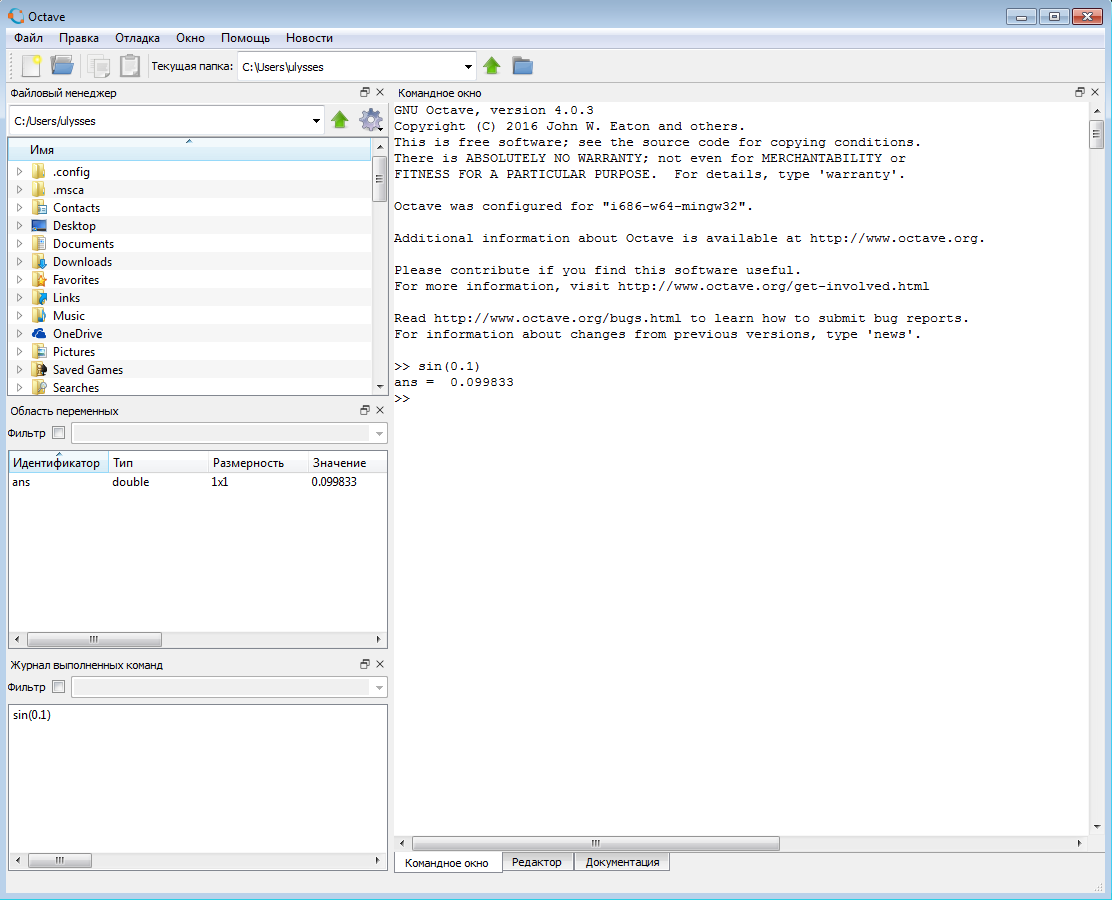
\includegraphics[width=0.7\textwidth]{octave.png}		
	\end{figure}
\end{frame}



\section{Основы работы в MATLAB}

\begin{frame}[fragile]{Окно программы}
  \begin{itemize}
    \item {\tt Command window} -- окно команд;
    \item {\tt Command history} -- окно истории истории команд;
    \item {\tt Current directory} -- окно, содержащие список файлов и папок текущего каталога;
    \item {\tt Editor} -- текстовый редактор.
    \item {\tt Workspace} -- окно со списком переменных текущей сессии.
  \end{itemize}
\end{frame}

\mode<all>
{
\usebackgroundtemplate{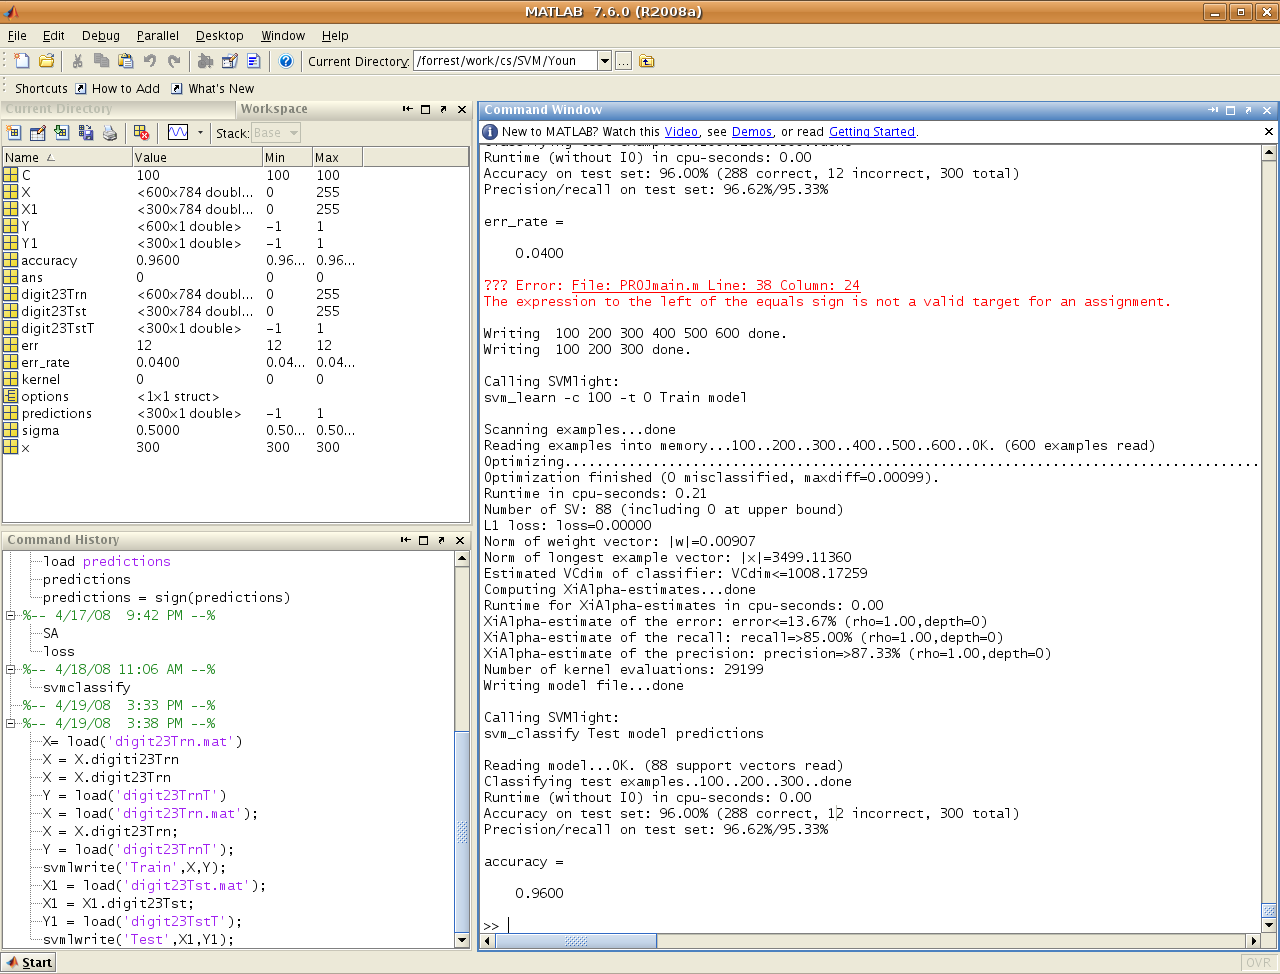
\includegraphics[width=1\paperwidth]{MATLAB-R2008a-for-Linux.png}}
\begin{frame}[plain]
\end{frame}
}
\mode<all>{\usebackgroundtemplate{}}
\mode*

\begin{frame}[fragile]{MATLAB как калькулятор}
\begin{itemize}
\item \matcode{a=1.2} -- присвоение  некоторого значения переменной \matcode{a} 
\begin{lstlisting}
>> a=1.2
a = 1.2
\end{lstlisting}
  \item \matcode{b=sin(a)*sqrt(a+2)} -- вычисление выражения и вывод результата
\begin{lstlisting}
>> b=sin(a)*sqrt(a+2)
b =
    1.6673
\end{lstlisting}
  \item \matcode{;} -- точка с запятой в конце выражения подавляет вывод результата:
\begin{lstlisting}
>> b=sin(a)*sqrt(a+2);
>>
\end{lstlisting}
\end{itemize}


\end{frame}
\begin{frame}[fragile]{Базовые команды редактора (Command window)}
  \begin{itemize}
    \item \matcode{$\uparrow$} -- возврат к предыдущей команде.
    \item \matcode{help имя функции} -- справка по функции (или F1).
    \item \matcode{cls} -- очистить окно команд (Command window).
    \item \matcode{clear} -- удалить все переменные в текущей сессии.
    \item \tikz \node [cbutton] {Ctrl}; \tikz \node [cbutton] {C};  - (в окне команд) прерывание вычислений.
  \end{itemize}
\end{frame}


\begin{frame}[fragile]
\frametitle{Синтаксис}
\begin{itemize}
\item Имена переменных могут состоять из латинских букв, цифр, знаков подчёркивания: \matcode{a, a1, x1, x\_1}. Имена переменных чувствительны к регистру: \matcode{A} и\matcode{a} -- это разные переменные.
\item При создании переменной может быть явно указан тип (по умолчанию \matcode{double}):
\begin{lstlisting} 
>> a=int16(25);
\end{lstlisting}
\end{itemize}  
\end{frame}



\begin{frame}[fragile]{Типы данных}
\begin{table}
\begin{tabular}{@{}ll@{}}
\toprule
Тип & Описание \\
\cmidrule{1-2}
\matcode{double} & вещественный, 64 бит \\
\matcode{single} & вещественный, 32 бит  \\
\matcode{int8} & знаковый целочисленный, 8 бит  \\
\matcode{int16} & знаковый целочисленный, 16 бит \\
\matcode{int32} & знаковый целочисленный, 32 бит \\
\matcode{int64} & знаковый целочисленный, 64 бит \\
\matcode{uint8} & беззнаковый целочисленный, 8 бит \\
\matcode{uint16} & беззнаковый целочисленный, 16 бит \\
\matcode{uint32} & беззнаковый целочисленный, 32 бит \\
\matcode{uint64} & беззнаковый целочисленный, 64 бит \\
\bottomrule
\end{tabular}
\end{table}
\end{frame}

\begin{frame}[fragile]
  \frametitle{Синтаксис}
  \begin{itemize}
    \item Квадратные скобки используются для создания векторов и матриц: \matcode{a=[1,2,3,4]}.
    \item Круглые скобки используются для вызова функций и для группировки выражений: \matcode{sin(1.2)+a*(c+1)}.  
    \item Фигурные скобки для создания массивов ячеек: \matcode{a=\{'Масса',10\}}
  \end{itemize}  
\end{frame}



% \begin{frame}[fragile]{Создание последовательностей}
% \begin{itemize}
%   \item \matcode{var=начальное значение:шаг:конечное значение}
%   по умолчанию шаг равен +1
% \begin{lstlisting}[frame=single]
% >> c = 1:2:10
% c =
%      1     3     5     7     9
% \end{lstlisting}
% Создание вектора-столбца
% \begin{lstlisting}
% >> c=(1:2:10)'
% c =
%      1
%      3
%      5
%      7
%      9
% \end{lstlisting}
% \end{itemize}
% \end{frame}


\begin{frame}[fragile]{Управление переменными}
  \begin{itemize}
    \item \matcode{whos} показать переменные текущей сессии
\begin{lstlisting}
>> whos
  Name      Size            Bytes  Class     Attributes

  a         1x1                 8  double              
  ans       1x5                40  double              
  b         1x1                 8  double              
\end{lstlisting}
    \item \matcode{clear} удалить все переменные текущей сессии
    \item \matcode{clear f1,f2} удалить переменные \verb|f1,f2| текущей сессии 
  \end{itemize}
\end{frame}

\begin{frame}[fragile]{Ведение ``протокола'' работы}  
  \begin{itemize}
    \item \matcode{diary filename} -- ведет запись на диск всех команд в строках ввода и полученных результатов в виде текстового файла.
    \item \matcode{diary off} -- приостанавливает запись в файл.
    \item \matcode{diary on} --  вновь начинает запись в файл.
  \end{itemize}  
\end{frame}

\begin{frame}[fragile]{Сохранение сессии}  
  Сохранение значения всех переменных в файл \matcode{*.mat}
  \begin{itemize}
    \item \matcode{save filename} -- запись в файл \alert{filename.mat} текущей сессии (значение всех переменных).
    \item \matcode{load filename} -- загрузка значений переменных из файла \alert{filename}.
  \end{itemize}
\end{frame}

\begin{frame}[fragile]{Ввод чисел}
\begin{tabbing}
    \matcode{a=1.25}  \hspace{75pt} \=  \\
    \matcode{a=9.3e10} \> $9.3 \cdot 10^{10}$\\
    \matcode{a=2.36e-5} \> $2.36 \cdot 10^{-5}$ 
\end{tabbing} 
\begin{lstlisting}    
>> a=1.25
a =  1.2500  
\end{lstlisting}    
\begin{lstlisting}    
>> a=9.3e10
a =    9.3000e+10
\end{lstlisting}    
\begin{lstlisting}    
>> a=2.36e-5
a =    2.3600e-05
\end{lstlisting}    
\end{frame}

\begin{frame}[fragile]{Формат отображения результата}
\begin{lstlisting}
>> format short;
>> pi 
ans=
   3.1416
\end{lstlisting}   
\begin{lstlisting}
>> format long;
>> pi 
ans=
   3.141592653589793
\end{lstlisting}   
\begin{lstlisting}
>> format short e;
>> pi 
ans=
   3.1416e+00
\end{lstlisting}   
\begin{lstlisting}
>> format long e;   
>> pi 
ans=
   3.141592653589793e+00   
\end{lstlisting}   
\end{frame}


\begin{frame}[fragile]{Константы}
  \begin{itemize}
    \item \matcode{pi} -- число $\pi$ 
\begin{lstlisting}
>> pi
ans =  3.1416  
\end{lstlisting}
    \item \matcode{realmin} -- минимальное положительное число 
\begin{lstlisting}
>> realmin
ans =   2.2251e-308
\end{lstlisting}
    \item \matcode{realmax} -- максимальное положительное число
\begin{lstlisting}
>> realmax
ans =   1.7977e+308
\end{lstlisting}    
  \end{itemize}
\alert{Использование имен переменных, совпадающих со встроенными именами, не рекомендуется}
\end{frame}

\begin{frame}[fragile]{Комплексные числа}
\begin{itemize}  
  \item \matcode{complex(1,3)} -- комплексное число $1+3i$
\begin{lstlisting}
>> a = complex(1,3);
\end{lstlisting}
  \item \matcode{i или j} -- мнимая единица $\sqrt{-1}$
\begin{lstlisting}
>> b = 1+2i;
>> a*b
ans =
  -5.0000 + 5.0000i
\end{lstlisting}
$$
  (1+3i)\cdot(1+2i) = 1 + 2i + 3i - 6 = -5 + 5i
$$
\end{itemize}
\end{frame}

\begin{frame}[fragile]{ans -- результат вычисления предыдущего действия}
Встроенная переменная \matcode{ans} хранит результат последнего действия:
\begin{lstlisting}
>> 2+2
ans =
   4
\end{lstlisting}  
Эту переменную можно использовать в выражениях:
\begin{lstlisting}
>> ans*5
ans =
   20
\end{lstlisting}    
\end{frame}


\begin{frame}[fragile]{Типы данных: векторы}
  \matcode{[1.2  1.5  1.9  0.5]} или \matcode{[1.2, 1.5, 1.9, 0.5]} вектор-строка \\
  $$\begin{bmatrix}1.2 & 1.5 & 1.9 & 0.5 \end{bmatrix}$$
  \matcode{[1.2; 1.5; 1.9; 0.5]} вектор-столбец \\
  $$\begin{bmatrix}1.2 \\ 1.5 \\ 1.9 \\ 0.5 \end{bmatrix}$$
\end{frame}

\begin{frame}[fragile]{Матрицы и скаляры}
Каждая переменная в MATLAB -- это матрица, поэтому переменная 
\begin{lstlisting}
>> a=1;
\end{lstlisting}
это матрица размерности 1x1:
\begin{lstlisting}
>> a(1,1)
ans =
   1
\end{lstlisting}  
\end{frame}

\begin{frame}[fragile]{Типы данных: матрицы}
  \begin{itemize}
   \item \matcode{A=[1.2  1.5  1.9; 0.5 0.6 0.7; 0.1 1 3]} \\
  $$\boldsymbol A=\begin{bmatrix}1.2 & 1.5 & 1.9 \\ 0.5 & 0.6 & 0.7 \\ 0.1 & 1 & 3\end{bmatrix}$$
   \item элементы вводятся построчно;
   \item элементы матрицы в строке можно разделять пробелами или запятыми;
   \item для разделения строк используются точка с запятой;
   \item элемент матрицы может быть числом или выражением.
  \end{itemize}
\end{frame}

\begin{frame}[fragile]{Выражение, как элемент матрицы}
\begin{lstlisting}
>> a = [1 2 3];
>> b = [7 8 9];
\end{lstlisting}  

\begin{lstlisting}
>> c = [a b*2]
>> c =
        1  2  3  14 16 18
\end{lstlisting}        

\begin{lstlisting}
>> c = [a; b+1]
>> c =
        1  2  3
        8  9  10
\end{lstlisting}
\end{frame}


% -----------------------------------------------------------------------------
\section{Операторы}
% -----------------------------------------------------------------------------
\begin{frame}[fragile]{Оператор ()}
  \matcode{help ops} вывести список всех операторов \\ \vspace{10pt}
\begin{verbatim}
  Operators and special characters.
 
  Arithmetic operators.
    plus       - Plus                    +    
    uplus      - Unary plus              +    
    minus      - Minus                   -    
    uminus     - Unary minus             -    
    mtimes     - Matrix multiply         *    
    times      - Array multiply         .*        
    power      - Array power            .^    
    ...
\end{verbatim}    
\end{frame}

\begin{frame}[fragile]{Оператор ()}
  \begin{itemize}
  \item \matcode{(i,j,k,...)} -- доступ к элементам матрицы.
  \item \matcode{A(i,j)} -- $i$ строка, $j$ столбец.  
  \item \matcode{A(i)} -- $i$ элемент вектора (строки или столбца) или $i$ элемент матрицы, при расположении элементов по столбцам.
  \end{itemize}
  \begin{figure}[ht]
  \centering
  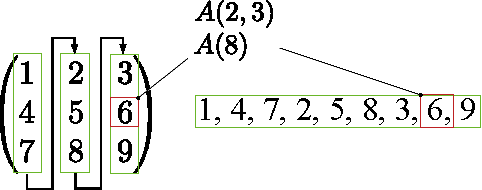
\includegraphics{./mat-get-element-op.pdf}
  % mat-get-element-op.pdf: 231x91 pixel, 72dpi, 8.15x3.21 cm, bb=0 0 231 91
  \end{figure}
\end{frame}

\begin{frame}[fragile]{Оператор \ : \ все элементы}
  Для прямоугольной матрицы $A$:
  \begin{itemize}
    \item \matcode{A(:,k)} -- k-ый столбец матрицы А
    \item \matcode{A(k,:)} -- k-ая строка матрицы А
    \item \matcode{A(:,[2,4,5])} -- второй, четвертый и пятый столбец матрицы А
\begin{lstlisting}
>> a = magic(4)
a =
    16     2     3    13
     5    11    10     8
     9     7     6    12
     4    14    15     1
>> a([1 3],:)
ans =
    16     2     3    13 
     9     7     6    12 
\end{lstlisting}
  \end{itemize}
\end{frame}

\begin{frame}[fragile]{Блоки матриц}
\matcode{A(1:2,3:4)} -- блок матрицы А, лежащий на пересечении строк 1 и 2, и столбцов 3 и 4.
\begin{lstlisting}
>> a = magic(4)
a =
    16     2     3    13
     5    11    10     8
     9     7     6    12
     4    14    15     1
>> a([1 2],[3 4])
ans =
     3    13
    10     8
\end{lstlisting}
\end{frame}

\begin{frame}[fragile]{Оператор \ :}
  \begin{itemize}
   \item Для создания списков с равноотстоящими значения используется оператор \matcode{:} \\ \matcode{n1:s:n2} \ \ $n1,n1+s,n1+2s,\ldots,n_k, \ n_k \leq n2$
   \item Оператор \matcode{:} может использоваться для доступа к элементам матрицы и вектора
   \item \matcode{A=1:10} \ -- \ $1,2,3,4,5,6,7,8,9,10$
   \item \matcode{A(1:2:10)} \ -- \ нечетные элементы вектора: \matcode{[1,3,5,7,9]}
  \end{itemize}
\end{frame}

\begin{frame}[fragile]{Удаление строк и столбцов из матрицы}
\matcode{A(3,:)=[]} -- удалить третью строку из матрицы $A$
\begin{lstlisting}
>> a = magic(4)
a =
    16     2     3    13
     5    11    10     8
     9     7     6    12
     4    14    15     1
>> a(3,:) = []
a =
    16     2     3    13
     5    11    10     8
     4    14    15     1
\end{lstlisting}
\end{frame}

\begin{frame}[fragile]{Последний элемент}
\begin{lstlisting}
>> a = [1,2,3 
        4,5,6];
>> a(end,:)
    
   4   5   6 

>> a(end-1,:)
    
   1   2   3 

>> a(end:-1:1,:)   

   4   5   6
   1   2   3 
\end{lstlisting}
\end{frame}  


\begin{frame}[fragile]{Логическое индексирование}
Логическое индексирование позволяет выбрать из вектора или матрицы элементы, удовлетворяющие заданному условию.
\begin{lstlisting}
>> a = sin(1:0.5:5)
a =
    0.8415    0.9975    0.9093    0.5985    0.1411   -0.3508   -0.7568   -0.9775   -0.9589
\end{lstlisting}
\begin{lstlisting}
>> ind=a<0
ind =
     0     0     0     0     0     1     1     1     1
\end{lstlisting}
\begin{lstlisting}
>> a(ind)   
ans = 
    -0.3508   -0.7568   -0.9775   -0.9589
\end{lstlisting}
\end{frame}

\begin{frame}[fragile]{Логическое индексирование для матриц}
\begin{lstlisting}
>> A = [1 2; 5 6]

A =
     7     2
     1     9
\end{lstlisting}
\begin{lstlisting}
>> ind=A>30

ind =
     1     0
     0     1
\end{lstlisting}
\begin{lstlisting}
>> A(ind)   

ans = 
    7
    9
\end{lstlisting}
\end{frame}

\begin{frame}[fragile]{Логические операторы < > = >= <= \textasciitilde =}  
  Результатом операции над матрицей или вектором является логический вектор (матрица):
  \begin{lstlisting}  
  >> A=[1,2,3,4,5,6];
  >> A<5  
  ans=
     [1,1,1,1,0,0]
  >> A==3
  ans=
     [0,0,1,0,0,0]
  >> A~=5   
  ans=
     [1,1,1,1,0,1]
  \end{lstlisting}   
\end{frame}

\begin{frame}[fragile]
\frametitle{Скалярное произведение векторов}
$$
\vec a \cdot \vec b = |a||b|\cos \varphi = a_x b_x + a_y b_y + a_z b_z
$$
Вычисление скалярного произведения, используя встроенную функцию \matcode{dot}:

\begin{lstlisting}[frame=single]
>> a=[1 2 3];
>> b=[4 5 6]; 
>> dot(a,b) 
ans =  
    32   
\end{lstlisting} 

\end{frame}

\begin{frame}[fragile]{Скалярное произведение векторов}
$$
\vec a \cdot \vec b = |a||b|\cos \varphi = a_x b_x + a_y b_y + a_z b_z
$$
Вычисление скалярного произведения, используя оператор матричное умножение:
\begin{lstlisting}[frame=single]
>> a*b'
ans =
    32 
\end{lstlisting}
\end{frame}

\begin{frame}[fragile]{Матричное умножение}
\matcode{A*B} умножение чисел или матриц (матричное умножение) 
\begin{lstlisting}
>> a = [1 2 3
        4 5 6];
>> b = [1 2
        3 4 
        5 6]; 
>> a*b
ans =
    22    28
    49    64
\end{lstlisting}   
\end{frame}

\begin{frame}[fragile]{Поэлементное умножение}
\matcode{C=A.*B} поэлементное умножение матриц $C_{ij}=A_{ij} B_{ij}$ 
\begin{lstlisting}
>> a = [1 2; 
        3 4];
>> b = [4 7;
        1 3];
>> a.*b
ans =
     4    14
     3    12  
\end{lstlisting}
\end{frame}

\begin{frame}[fragile]{Возведение в степень}
Возведение в степень матрицы или числа 
\begin{lstlisting}
>> a=[1 2
      3 4];
>> a^2
ans =
     7    10
    15    22   
\end{lstlisting}
$$
  \boldsymbol a^2 = \boldsymbol a \cdot \boldsymbol a = 
  \begin{pmatrix} 1 & 2 \\ 3 & 4 \end{pmatrix} \cdot \begin{pmatrix} 1 & 2 \\ 3 & 4  \end{pmatrix} = \begin{pmatrix} 7 & 10 \\ 15 & 22 \end{pmatrix}
$$
\end{frame}

\begin{frame}[fragile]{Возведение в степень}
Возведение в степень всех элементов матрицы
\begin{lstlisting}
>> a=[1 2
      3 4];
>> a.^2
ans =
     1     4
     9    16   
\end{lstlisting}
\end{frame}

\begin{frame}[fragile]{Операторы}
  \begin{itemize}
   \item \matcode{A'} -- транспонирование матрицы:
\begin{lstlisting}
>> A=[1.2 0.3;
      0.5 2.1];
>> A'
ans =
    1.2000    0.5000
    0.3000    2.1000
\end{lstlisting}   
   \item \matcode{C=A/B} -- деление $C=A B^{-1}$
   \item \matcode{C=A./B} -- поэлементное деление $C_i=A_i / B_i$ \\
  \end{itemize}
\end{frame}

\begin{frame}[fragile]{Решение системы линейных уравнений}
  Деление \matcode{A\textbackslash B} выполняет операцию $\boldsymbol C=\boldsymbol A^{-1} \boldsymbol B$ -- решение СЛУ с матрицей коэффициентов $\boldsymbol A$ и матрицей правой части $\boldsymbol B$:
$$
\left\{
\begin{aligned}
  & 1.2 x_1 + 0.3 x_2 = 1; \\
  & 0.5 x_1 + 2.1 x_2 = 2.
\end{aligned}  
\right.
$$
\begin{lstlisting}
>> A=[1.2 0.3;0.5 2.1];
>> B=[1;2];
>> A\B
ans =
    0.6329
    0.8017
\end{lstlisting}
\end{frame}





% %
% %
% %
% %
% \section{Задачи}
% %
% %
% %
% %

% \begin{frame}[c]{Задание 1}
% Напишите кратчайшее однострочное выражение для построения квадратной матрицы вида
%   $$
%   \begin{bmatrix}
%    1 & 2 & 3 & 4 & \ldots & n \\
%    1 & 2 & 3 & 4 & \ldots & n \\
%    \ldots & \ldots & \ldots & \ldots & \ldots & n \\
%    1 & 2 & 3 & 4 & \ldots & n
%   \end{bmatrix}
%   $$
% \end{frame}

% \begin{frame}[c,fragile]{Задание 2}
% Напишите выражение, определяющее индекс элемента вектора с наименьшим отклонением от среднего значения элементов вектора $\mathbf P$
% $$ 
%   i: \text{min }|P_i-m(\mathbf P)|
% $$
% Например, для 
% $$ P = [8,1,2,2,0,3] $$
% ответом будет $6$, т.е. шестой элемент массива находится ближе всего к среднему значению элементов массива. Среднее значение определяется при помощи функции \emphb{mean}
% \begin{lstlisting}
% >> P=[8 1 2 2 0 3];
% >> mean(P)
% ans =  2.6667
% >>
% \end{lstlisting}

% \end{frame}

% \begin{frame}[c]{Задание 3}
% Напишите код, который находит матрицу $\mathbf B$, отличающуюся от матрицы $\mathbf A$ перестановкой столбцов по возрастанию суммы элементов столбца.
% $$
%   \mathbf A = 
%   \begin{bmatrix}
%     2 & 3 & 5 \\
%     4 & 1 & 9 \\
%     3 & 0 & 2
%   \end{bmatrix} \quad \Rightarrow \quad 
%   \mathbf B = 
%   \begin{bmatrix}
%     5 & 2 & 3 \\
%     9 & 4 & 1 \\
%     2 & 3 & 0
%   \end{bmatrix}
% $$
% $$
%   \boxed{5 + 9 + 2} > \boxed{2 + 4 + 3} > \boxed{3 + 1 + 0}
% $$
% \end{frame}


% \begin{frame}[fragile]{Задание 4}
% В матрице $\mathbf A$ записаны координат точек на плоскости: в первом столбце --  координаты $x$, во втором столбце -- $y$:
% $$
%   \boldsymbol A = \begin{bmatrix} x_1 & y_1 \\ x_2 & y_2 \\ x_3 & y_3 \\ \ldots & \ldots \\ x_n & y_n \end{bmatrix}
% $$
% Постройте матрицу $\mathbf B$, которая составлена из строк матрицы $\mathbf A$ так, что с увеличением номера строки с координатами точки растёт расстояние от этой точки до начала координат.
% \end{frame}


% \begin{frame}[fragile]{Задание 5}
% \begin{columns}
% \column{.2\textwidth}
% \begin{center}
% \begin{tikzpicture}[vertex/.style={circle,minimum width=7mm,thick,draw=red!50!black!50,
% top color=white,bottom color=red!50!black!30}]
% \node[vertex] (1) {$1$};
% \node[vertex] (2) at (-1.0,1) {$2$};
% \node[vertex] (4) at (-1.3,3) {$4$};
% \node[vertex] (3) at (0,3) {$3$};
% \path[-] (1) edge (2);
% \path[-] (2) edge (4);
% \path[-] (4) edge (3);
% \end{tikzpicture}
% \end{center}
% \column{.8\textwidth}
% Структура графа описана при помощи списка смежности, записанного в виде матрицы:
% $$
% \mathbf L = \begin{bmatrix}
%      1 & 2 \\
%      2 & 4 \\
%      \ldots & \ldots \\
%      3 & 4 \\
%     \end{bmatrix},
% $$

% В каждой строке матрицы $\mathbf L$ записываются индексы вершин, связанные дугой.
% \\ Постройте матрицу смежности графа $\mathbf S$, элемент которой -- $s_{ij}$ отличен от нуля, только если вершины $i$ и $j$ смежные, т.~е. соединены дугой. Остальные элементы матрицы $\mathbf S$ равны нулю.
% \end{columns}
% \end{frame}

\end{document}
